Una volta concluso lo sviluppo del GRIDS System con Blockchain integrata, è indispensabile valutarne le performance.

La metrica che è stata adoperata per la misura delle prestazioni della piattaforma è il ritardo, nello specifico, sono stati misurati tre tipi di delay:

\begin{itemize}
    \item \textit{End-to-end delay}: il tempo che intercorre tra il momento in cui il client effettua la richiesta di dati e quello in cui la transazione viene confermata e l'utente può visualizzare i dati;
    \item \textit{Client-side delay}: il lasso di tempo tra l'invio della richiesta da parte del Client e la ricezione della risposta da parte del Server con l'indirizzo al quale saranno disponibili i dati una volta confermata la transazione;
    \item \textit{Instant buy delay}: l'intervallo di tempo necessario per la ricezione dei dati a partire dalla richiesta di dati con credito residuo.
\end{itemize}

Una considerazione molto importante da fare è che, nel caso delle transazioni "lente", vi è una sorta di problema di "campionamento": visto che nella Testnet i blocchi vengono estratti ogni circa 20 minuti (che scende a 10 nel caso della rete Bitcoin ufficiale), il tempo di ritardo varierà in base a quanto tempo prima è stato risolto l'ultimo blocco della blockchain.

La prima prova è stata effettuata con 100 transazioni standard, però alcune di esse sono state respinte per "error 64: too-long-mempool-chain". Per spiegare efficacemente questo tipo di errore, è necessario introdurre il concetto di \textit{mempool}.
Il Mempool (\textit{memory pool}) consiste nell'insieme di transazioni in attesa di approvazione da un miner. Ogni nodo della rete Bitcoin ha il proprio mempool, e quindi avrà una certa dimensione, rappresentata nell'ordine dei megabyte.

Ciò vuol dire che, se viene generata una grande quantità di transazioni, il mempool può costituire un bottleneck se non gestito opportunamente: nel caso della rete Bitcoin, in questi casi alcune transazioni generate possono venire rifiutate, come effettivamente si è verificato durante il primo test.

In Bitcoin Core\footnote{https://bitcoin.org/en/bitcoin-core/} il limite di transazioni che possono "sostare" nel mempool è di 25, anche se questo numero è generalmente soggetto a variazioni. Con bitcoinj non è stato implementato un modo per aggirare questo limite perchè, visto che i nodi sono in modalità SPV, e ciò va in antitesi con la capacità di generare un numero molto grande di transazioni.

In ogni caso la piattaforma possiede il meccanismo di recharge, quindi il problema viene aggirato in maniera semplice ed efficace.

%%
Un'altra importante precisazione da fare è che il mempool error si può verificare quando è un singolo wallet a generare troppe transazioni di seguito, non quando sono tanti wallet a generare meno transazioni: ciò significa che la rete SIoT non costituisce \textit{bottleneck}. In condizioni di utilizzo normale da parte di un utente qualsiasi, difficilmente saranno mandate così tante richieste
%%

La prima prova ha dato dei risultati per quato riguarda il delay end-to-end e quello client-side, dei quali sono rappresentate rispettivamente le CDF, ossia la distribuzione cumulativa di probabilità, nelle figure \ref{f:calcoli:end2end} e \ref{f:calcoli:client}. 

\begin{figure}[h!t]
\centerline{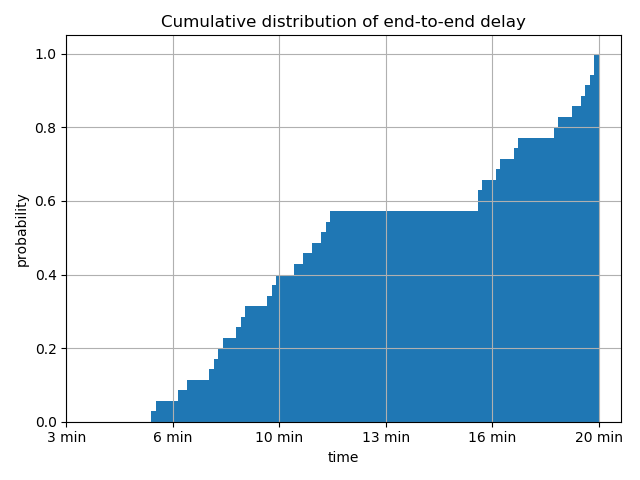
\includegraphics[width=\textwidth]{img/end-to-endGIUSTO}}
\caption{CDF dei delay end-to-end delle transazioni}
\label{f:calcoli:end2end}
\end{figure}

Il client-side delay tende ad assumere una distribuzione normale: il grafico, infatti, ricorda molto quello di una \textit{normal function}. 
L'end-to-end delay, invece, presenta valori temporali molto più ampi, visto che è compreso il tempo della conferma delle transazioni. La discontinuità che si osserva nel grafico è causata dal fatto che una parte delle transazioni sono state incluse in un blocco, mentre un'altra parte è stata confermata nel blocco successivo. Da notare, inoltre, che il gradino presenta una durata di 5 minuti anzichè di 20, come ci si aspetterebbe dal tempo medio di creazione dei blocchi.

\begin{figure}[h!t]
\centerline{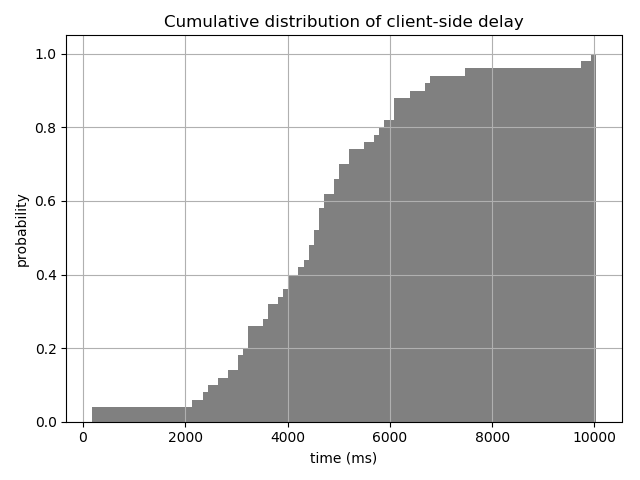
\includegraphics[width=\textwidth]{img/client-side-delay-grey}}
\caption{CDF dei delay client-side delle transazioni}
\label{f:calcoli:client}
\end{figure}

Le instant buy, infatti, presentano ritardi molto contenuti, com'era auspicabile. Da notare che il punto con ritardo più alto corrisponde alla prima richiesta.

Infine, confrontando i valori temporali delle transazioni standard e delle instant buy, si può osservare un considerevole aumento delle performance, nello specifico del 99\%.

\begin{figure}[h!t]
\centerline{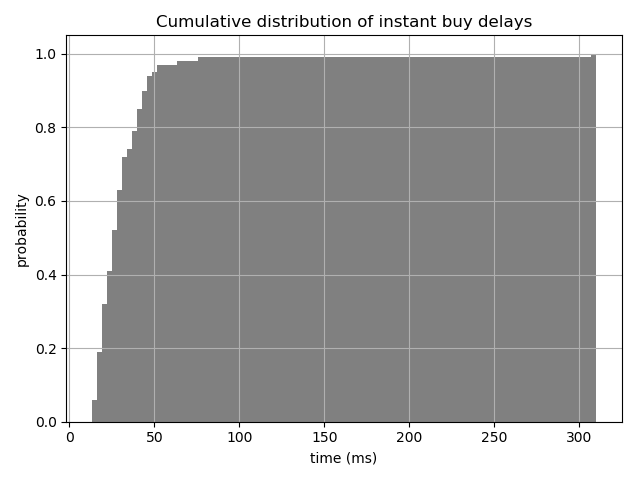
\includegraphics[width=\textwidth]{img/instant-buy-delay-grey}}
\caption{CDF dei delay delle transazioni effettuate con credito}
\label{f:calcoli:instant}
\end{figure}

